% Chapter Template

\chapter{zCash and zk-SNARKs} % Main chapter title

\label{Chapter3} % Change X to a consecutive number; for referencing this chapter elsewhere, use \ref{ChapterX}

%----------------------------------------------------------------------------------------
%	SECTION 1
%----------------------------------------------------------------------------------------

\section{zCash}

Cryptocurrencies have appeared recently and have been marketed as an alternative to cash and electronic payments. The best example is the Bitcoin bubble which made people gain millions overnight, and lose them soon after. However, Bitcoin is of limited use today. It cannot be used as a general currency due to the low throughput and long waiting times for the transaction to be added to the block. Its status as an anonymous currency is also disputed, resulting in 2 different cryptocurrencies being developed to fill that void - Monero (XMR) \cite{monero} and zCash (ZEC) \cite{zcashmain}.\\
\\
ZCash defines two types of addresses. Transparent addresses behave the same way as Bitcoin addresses. Data resides in the public blockchain so it can be tracked the same way as with Bitcoin. However, shielded addresses reveal nothing when they are a part of the transaction. This is accomplished by using notes (\textbf{NOTE}) which contain the public key (\textbf{PK}) of the owner, some amount of zCash (\textbf{M}), as well as a unique identifier (\textbf{N}). Every shielded transaction results in a note like this (transaction output). When this note is used in a transaction, it is spent, and its nullifier (\textbf{NULL(N)}) is published. Valid, unspent notes are ones which are in the set of all generated notes, and whose nullifier hasn't been published.\\
\\
Keeping all notes in a list would result is an abysmal performance, so they are kept in a Merkle tree. Furthermore, instead of keeping notes in a public structure, where everyone can see them, we keep commitments to notes (\textbf{COMM(NOTE)}). This guarantees that the value and owner of note are not public. However, now that we don't know \textbf{PK} of the note's owner, how do we verify the transaction?\\
\\
Spending a note in zCash involves computing a zero-knowledge proof $\pi$. This requires the \textbf{NOTE}'s spender to prove the following:

\begin{itemize}
    \item The commitment \textbf{COMM(NOTE)} exists in a Merkle tree with all notes
    \item That they have the private key \textbf{SK}, corresponding to the note's public key \textbf{PK}
    \item The \textbf{NULL(N)} is equal to the nullifier provided (\textbf{T})
\end{itemize}

If the proof verification passes, the node can check if the note has been spent previously by searching for \textbf{T} in a Merkle tree with published nullifiers. This results in the transaction being accepted and added to the blockchain. Along with this \textbf{T} is added to the set of spent nullifiers. For more information read \cite{zcashzksnarks, zcashprotocol}.

%----------------------------------------------------------------------------------------
%	SECTION 2
%----------------------------------------------------------------------------------------

\section{Zero-Knowledge Proofs}

In 1985. Goldwasser, Micali, and Rackoff published a paper with an interesting twist \cite{goldwasser1985knowledge}. Most papers discussed methods of combating a dishonest prover, trying to deceive an honest verifier. Their work took a completely different approach: What information could a verifier obtain from a prover? They defined a new class of languages - IP (Interactive Proof). IP contains language L for which there is an interactive protocol between the prover P and a verifier V, after which P has convinced V with a non-negligible probability that the statement s is in the language L.\\
\\
The interactive proof must satisfy the following properties:
\begin{itemize}
    \item \textbf{Completeness} If the statement \textit{s} is in \textit{L}, there exists a prover \textit{P} that can convince the poly-time verifier \textit{V} of this, with probability of at least 2/3.
    $$ s \in L \implies \exists P Pr[out_V \langle V, P \rangle (s) = 1 ] \geq 2/3 $$
    \item \textbf{Soundness} If the statement \textit{s} isn't in \textit{L}, no prover \textit{P} can convince the poly-time verifier \textit{V} that it is with probability 1/3 or greater.
    $$ s \notin L \implies \forall P Pr[out_V \langle V, P \rangle (s) = 1 ] < 1/3 $$
\end{itemize}

The choice of constants 2/3 and 1/3 is arbitrary because probability amplification can be used until we are satisfied with the probability of error.\\
\\
Another important property that proof may have is \textbf{zero-knowledge}. While two previous properties are tied to different provers, zero-knowledge states that all verifiers can learn only that the statement \textit{s} belongs to the language \textit{L}. This statement can be formalized using a simulator and a transcript. \textit{V} can generate the transcript with the same distribution as the messages exchanged during the protocol, without ever communicating with \textit{P}. Hence, \textit{V} learns nothing from \textit{P}, other than $s \in L$.\\
\\
Unfortunately, zero-knowledge proofs described are interactive. They cannot be used in blockchain because every verification of the blocks would require all parties to be online and exchange messages with the verifier. Blum, Feldman and Micali \cite{blum1988non} introduced \textbf{N}on-\textbf{I}nteractive \textbf{Z}ero-\textbf{K}nowledge proofs (NIZK - pronounced \textit{nee-zeek}). These proofs require a preparation step - the establishment of a common reference string (CRS). This is performed once and CRS is later used for proof generation and verification.

\section{zk-SNARKs}

\subsection{Introduction}
zk-SNARKs are a cryptographic primitive used for zero-knowledge proofs. Their name stands for \textbf{Z}ero-\textbf{K}nowledge \textbf{S}uccinct \textbf{N}on-Interactive \textbf{Ar}guments of \textbf{K}nowledge. They cannot be considered true proofs, but arguments because they hold only computationally. The main strength lies in succinctness and non-interactivity - zk-SNARK proofs are short and can be verified offline. Furthermore, they can be used to prove any statement that can be represented as a circuit (eg. any finite computation on a modern CPU). This can be useful in a number of contexts, not only for cryptocurrencies. (eg. verifiable cloud execution). zk-SNARKs aren't interactive so they require a preparation stage to generate a CRS.\\
\\
Most of the material in this section is based on a series of articles by Vitali Buterin\cite{buterin1, buterin2, buterin3} and is meant to bridge the gap between Buterin's articles and full papers. The differences from Buterin's articles, as well as from the original papers are discussed at the end of this section. For further information consult original papers - Pinocchio protocol\cite{parno2013pinocchio} and Zerocash whitepaper \cite{sasson2014zerocash}, as well as zCash blog \cite{zcashzksnarks} and zCash protocol \cite{zcashprotocol}. % cite Pinocchio, Groth, zCash blog posts, articles by Vitali Buterin

\subsection{Arithmetic Circuit}

The calculation we want to perform starts as a program. To generate a proof for it, we need to convert it into an arithmetic circuit over the field $\mathbb{F}$. The gates in the circuit consist of two field operations and their inverses (eg. addition, multiplication, subtraction, and division). Different variables in the program and intermediate results are represented by different wires in the circuit. Conditional execution can be simulated by performing all branches in parallel, and selecting one of them. Finite loops are unrolled and function calls are inlined.

\subsection{R1CS Form}
The next step of generating a proof is making sure that all constraints in the circuit are satisfied (eg. that multiplication gates actually perform multiplication). This is achieved by conversion of the circuit into R1CS form (Rank 1 Constraint System). Every gate is transformed independently. It consists of a vector S, containing values of all wires in the circuit, with value 1 prepended to this vector. Additionally, R1CS form comprises vectors $A_i$, $B_i$, and $C_i$, such that the following constraint is met:

$$ A_i \cdot S \times B_i \cdot S - C_i \cdot S = 0 $$

The conversion follows a standardized procedure for all four basic operations, which is illustrated in Figure \ref{fig:r1csmul} for multiplication. Vectors A and B are used for selection and scaling of inputs to the gate, while the vector C scales and selects the output. We transform all gates as described. Due to the properties of dot product, we can also collapse all additions and subtractions into multiplication and division gates.

\begin{figure}[h]
    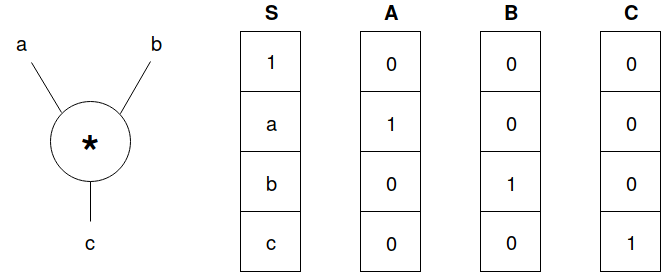
\includegraphics[width=\linewidth]{Figures/R1CS.png}
    \caption{Conversion of Multiplication to R1CS Form}
    \label{fig:r1csmul}
\end{figure}

\subsection{Quadratic Arithmetic Program}
Quadratic Arithmetic Program enables us to represent R1CS constraints for all gates at once. First, we enumerate all gates, and construct three polynomials (A(x), B(x), and C(x)) for every variable in the circuit. Polynomial for the j-th variable $A_j(x)$ is formed by interpolating it through the points with coordinates $(i, A_i[j])$. 
%, where GateIndex is the index assigned to gate when they were enumerated, $A_{GateIndex}$ is the corresponding A vector, and $A_{GateIndex} [i]$ is the value of the i-th constant in the vector
Polynomials can be interpolated using well-known algorithm such as Langrangian interpolation. Extracting previous values from the polynomial is possible by evaluating them at the corresponding variable index.\\
\\
Then, we form a new polynomial A(x) by arranging all $A_j$ vectors in a new vector based on the index j, and taking a scalar product with S. We form polynomials B(x) and C(x) the same way.

$$ A(x) = \sum_{j = 1}^{number\,of\,gates} S_j \cdot A_j(x) $$

Considering that polynomials A(x), B(x) and C(x) are sums of interpolated polynomials multiplied by the corresponding element in S, we can evaluate them at different indices and conclude that the following expression holds.

$$\forall t:\: [t \in \{1,\,2,\,3, \dots ,\,number\,of\,gates\} \implies A(t) \cdot B(t) - C(t) = 0]$$
\\
This implies that the polynomial $A(x) \cdot B(x) - C(x)$ is divisible by the polynomial $T(x) = (x-1)(x-2)...(x-number\,of\,gates)$, or more formally:

$$ A(x) \cdot B(x) - C(x) = H(x) \cdot T(x) $$

\subsection{Pinocchio Protocol}

This section presumes basic (operational) knowledge of elliptic curves and pairings. In his articles Buterin provides a decent, albeit non-technical, introduction to both elliptic curves and pairings \cite{buterin1, buterin2, buterin3}. For short black-box treatment of different cryptographic pairings, consult \cite{galbraith2008pairings}. Readers looking for a more textbook introduction to pairings, can read \cite{costello2012pairings}.\\
\\
The simplest way to verify that all checks that the circuit, or QAP, performs are satisfied, would be to reveal all values. However, that would leak sensitive information such as private key, available funds, transferred ZEC\dots Providing just a polynomial divisible by T(x) would be meaningless, because it could have been forged. The primitive we need should provide us with a way to check that the polynomial was constructed in a specific way, while letting us verify that it is indeed divisible by T(x). Pinocchio protocol \cite{parno2013pinocchio} uses  pairings (bilinear maps) to achieve that goal.\\
\\
In this section, we use type III pairing: $e: \mathbb{G}_1 \times \mathbb{G}_2 \to \mathbb{G}_T$. Pairing is denoted by a two-argument function $e(P_{G_1}, P_{G_2})$. $G_1, G_2$ and $G_T$ represent generators of groups $\mathbb{G}_1$, $\mathbb{G}_2$ and $\mathbb{G}_T$, respectively. All group operations are represented in the additive notation to stress that we are working with elliptic curve points (+ for the operations in $\mathbb{G}_1$ and $\mathbb{G}_2$, $\oplus$ for $\mathbb{G}_T$ , and $[n]P$ for scalar multiplication for all groups).\\
\\
Pairings can be used to check whether two pairs of elliptic curve points (A and B, C and D) have the same quotients:

$$ B / A \stackrel{?}{=} D / C $$
This is verified by computing two pairings:
$$ e(A, D) \stackrel{?}{=} e(B, C) $$
In case of $A = [k]B; C = [k]D$ we have:
$$ e([k]B, D) \stackrel{?}{=} e(B, [k]D)$$
We use property of the pairing to move the constant outside the pairings:
$$ [k]e(B, D) = [k]e(B, D) $$
If the pairs have the same quotients, both pairings will be equal.\\
\\
Using this idea, we can make sure that a polynomial hasn't been forged. We evaluate all polynomials at a secret coordinate t, so we obtain $A_j(t), B_j(t), C_j(t)$ for all gates in the circuit. By also adding these values multiplied by secret coefficients $k_a, k_b$ and $k_c$, we are able to prevent the prover from using arbitrary polynomials. Considering that pairings operate on elliptic curve points, we will use these values to multiply the generator point $G_1$ of a pairing-friendly curve. Values $\rho_A, \rho_B, \beta, \gamma$ are also considered secret, and are used to aid subsequent pairing checks. Accordingly, we add the following values to the trusted setup:

$$\forall j \in \{1, 2, 3, \ldots, number\;of\;gates\} : [\rho_A A_j(t)]G, [k_A \rho_A A_j(t)]G_1 $$
$$\forall j \in \{1, 2, 3, \ldots, number\;of\;gates\} : [\rho_B B_j(t)]G, [k_B \rho_B B_j(t)]G_1 $$ 
$$\forall j \in \{1, 2, 3, \ldots, number\;of\;gates\} : [\rho_C C_j(t)]G, [k_C \rho_C C_j(t)]G_1 $$ 

The prover then needs to provide the following points to prove that they computed polynomials $A(x), B(x), C(x)$ correctly:

$$\pi_A = [\rho_A A(t)]G_1, \pi_A' = [k_A \rho_A A(t)]G_1$$
$$\pi_B = [\rho_B B(t)]G_2, \pi_B' = [k_B \rho_B B(t)]G_1$$
$$\pi_C = [\rho_A \rho_B C(t)]G_1, \pi_C' = [k_C \rho_A \rho_B C(t)]G_1$$

The check is performed by computing:

$$ e(\pi_x, [k_x]G_2) \stackrel{?}{=} e(\pi_x', G_2) $$

Considering that polynomials $A(x), B(x), C(x)$ are linear combinations of polynomials $A_j(x), B_j(x), C_j(x)$, respectively, required points can be computed from the points in the trusted setup and the witness \textit{s} (\textit{s} represents the coefficients of linear combination).\\
\\
The prover must also convince the verifier that they have used the same coefficients for all polynomials. This is achieved by extending the trusted setup with the following points:

$$\forall j \in \{1, 2, 3, \ldots, number\;of\;gates\} : [\beta(\rho_A A_j(t) + \rho_B B_j(t) + \rho_A \rho_B C_j(t))]G_1 $$

The prover then provides the point:

$$ \pi_{K} = [\beta(\rho_A A(t) + \rho_B B(t) + \rho_A \rho_B C(t))]G_1 $$

Pairing check is performed by the verifier:

$$ e(\pi_K, [\gamma]G_2) \stackrel{?}{=} e(\pi_A + \pi_C, [\gamma\beta]G_2) \oplus e([\gamma\beta]G_1, \pi_B) $$

Finally, they need to prove that the polynomial $A(x) \cdot B(x) - C(x)$ is really divisible by $T(x)$. This is achieved by using the polynomial $H(x)$ to show that multiplying it by $T(x)$ gives us $A(x) \cdot B(x) - C(x)$. If the prover provides $\pi_H = [H(t)]G_1$, we can do this using pairings:

$$ e(\pi_a, \pi_b) \stackrel{?}{=} e(\pi_c, G_2) \oplus e(P_H, [\rho_A \rho_B T(t)]G_2) $$

We will now discuss the simplifications made to the proof. The proof explained works for proofs without any input wires. Adding inputs to the circuit is straightforward. It involves introducing several terms to the CRS and adding them to $\pi_A$ during the linearity and divisibility checks. The reader can check the full version of Pinocchio zk-SNARKs in \cite{parno2013pinocchio}, or just the review at the end of \cite{ben2014succinct}.\\
\\
There is another important place where we deviate from Buterin's articles - pairing used. We use asymmetric pairing, instead of symmetric pairing used by Buterin. Asymmetric pairings are more efficient and make Groth's results in the section \ref{grothexpl} easier to understand.\\
\\
The final remark has to do with the choice of groups $\mathbb{G}_1$ and $\mathbb{G}_2$ for the points provided by the prover. All points beside $\pi_B$ are elements of $\mathbb{G}_1$. Elements of $\mathbb{G}_1$ are smaller than the elements of $\mathbb{G}_2$. Pinocchio protocol takes advantage of this to reduce the size of the proof by assign as many points as possible to $\mathbb{G}_1$. $\pi_B$ is the only point that has to be in $\mathbb{G}_2$ due to the pairing check where we calculate $e(\pi_A, \pi_B)$. This brings us to the proof consisting of 7 $\mathbb{G}_1$ and 1 $\mathbb{G}_2$ element.

\section{Sapling Update}

\subsection{Introduction}
zCash is undergoing continuous development. The most substantial update to date is called Sapling \cite{zcashsapling}. Its goal was to overhaul the cryptography of zCash. The major changes are a new curve, new commitment scheme, a new proving system, as well as writing these components in Rust. The changes are meant to address the slow speed of shielded transactions, and lead to their wider adoption.

\subsection{New Curve: BLS12-381}

The old curve BN254 saw its security level reduced after a new algorithm was discovered \cite{zcashbls12381}. Increasing the security parameters for this curve would reduce the performance of FFT (for polynomial division) and multiexponentiation steps of proof generation. A new curve was selected - BLS12-381. The embedding degrees of this curve is 12. Other parameters of this curve are its group order $r \approx 2^{255}$ and the base field characteristic $q \approx 2^{381}$.

\subsection{New Commitment Scheme: Pederson Commitments and JubJub}

zCash zk-SNARK circuit needs to compute and verify commitments to notes. SHA256 compression function was used as the commitment scheme. Unfortunately, this also bloated the circuit quite a bit. Moving to BLS12-381, whose group order is $r \approx 2^{255}$ was used to introduce a new commitment scheme: Pederson commitments over a custom Edwards curve Ed255-JubJub\cite{zcashjubjub}. The field underlaying JubJub can fit in the scalar field of BLS12-381 and be calculated in the circuit quite efficiently.

\subsection{New Proving System}
\label{grothexpl}

While Pinocchio is secure, its biggest problem is the proof size. Instead of using 7 $\mathbb{G}_1$ elements, and one $\mathbb{G}_2$ element, Jens Groth\cite{groth2016size} improved upon the previous work to use only 2 $\mathbb{G}_1$ elements and a $\mathbb{G}_2$ element. He also proved that at least one element needs to be in each group for linear circuit checks to be secure.\\
\\
The new system has the prover provide:

$$ \pi_A = [\underbrace{\alpha + A(t) + r\delta}_\text{X}]G_1 $$
$$ \pi_B = [\underbrace{\beta + B(t) + s\delta}_\text{Y}]G_2 $$
$$ \pi_C = [\frac{\beta A(t) + \alpha B(t) + C(t) + H(t)T(t)}{\delta} + Xs + Yr - rs\delta]G_1 $$

The verifier needs to check:

$$ e(\pi_A, \pi_B) \stackrel{?}{=} e(\alpha G_1, \beta G_2) \oplus e(\pi_C, \delta G_2) $$

Groth's zk-SNARK has been simplified here and doesn't include inputs to the circuit. Constants $\alpha, \beta, \delta, r, s, t$ are random secrets generated during the generation of CRS. Polynomials A(x), B(x), C(x), H(x), and T(x) are defined in the same way as in Pinocchio \cite{parno2013pinocchio} protocol.

\subsection{Rust Implementation}

Rust \cite{rustlang} was imagined as a memory-safe and thread-safe low-level programming language. Switching to a new curve required taw rewrite of the cryptographic code. This was done in Rust to improve the security of zCash \cite{zcashbellman}. Furthermore, new CRS was needed for Groth's proving system. The program for the ceremony was also written in Rust and used secure multiparty computation to guarantee honesty. 87 people contributed in the first (circuit-agnostic) phase, and over 90 took part in the second phase \cite{zcashparamgen}.